% ==============================================================================
% CAPÍTULO 5: DISEÑO DEL SISTEMA
% ==============================================================================

\section{Arquitectura general del sistema}

Para dar respuesta a los requisitos de bajo consumo, alta resiliencia y soberanía completa del dato analizados previamente, se ha diseñado e implementado una arquitectura integral de monitorización IoT extremo a extremo (\textit{End-to-End}). El sistema abarca desde la sensórica física de campo hasta la capa analítica de visualización web, desacoplando la adquisición y la persistencia mediante interfaces de comunicación estándar e infraestructuras desatendidas de código abierto.

En la Figura~\ref{fig:arquitectura_general} se ilustra el esquema global del sistema desarrollado, detallando la interconexión de los subsistemas hardware y las capas lógicas de procesamiento y transporte.

\begin{figure}[!htbp]
    \centering
    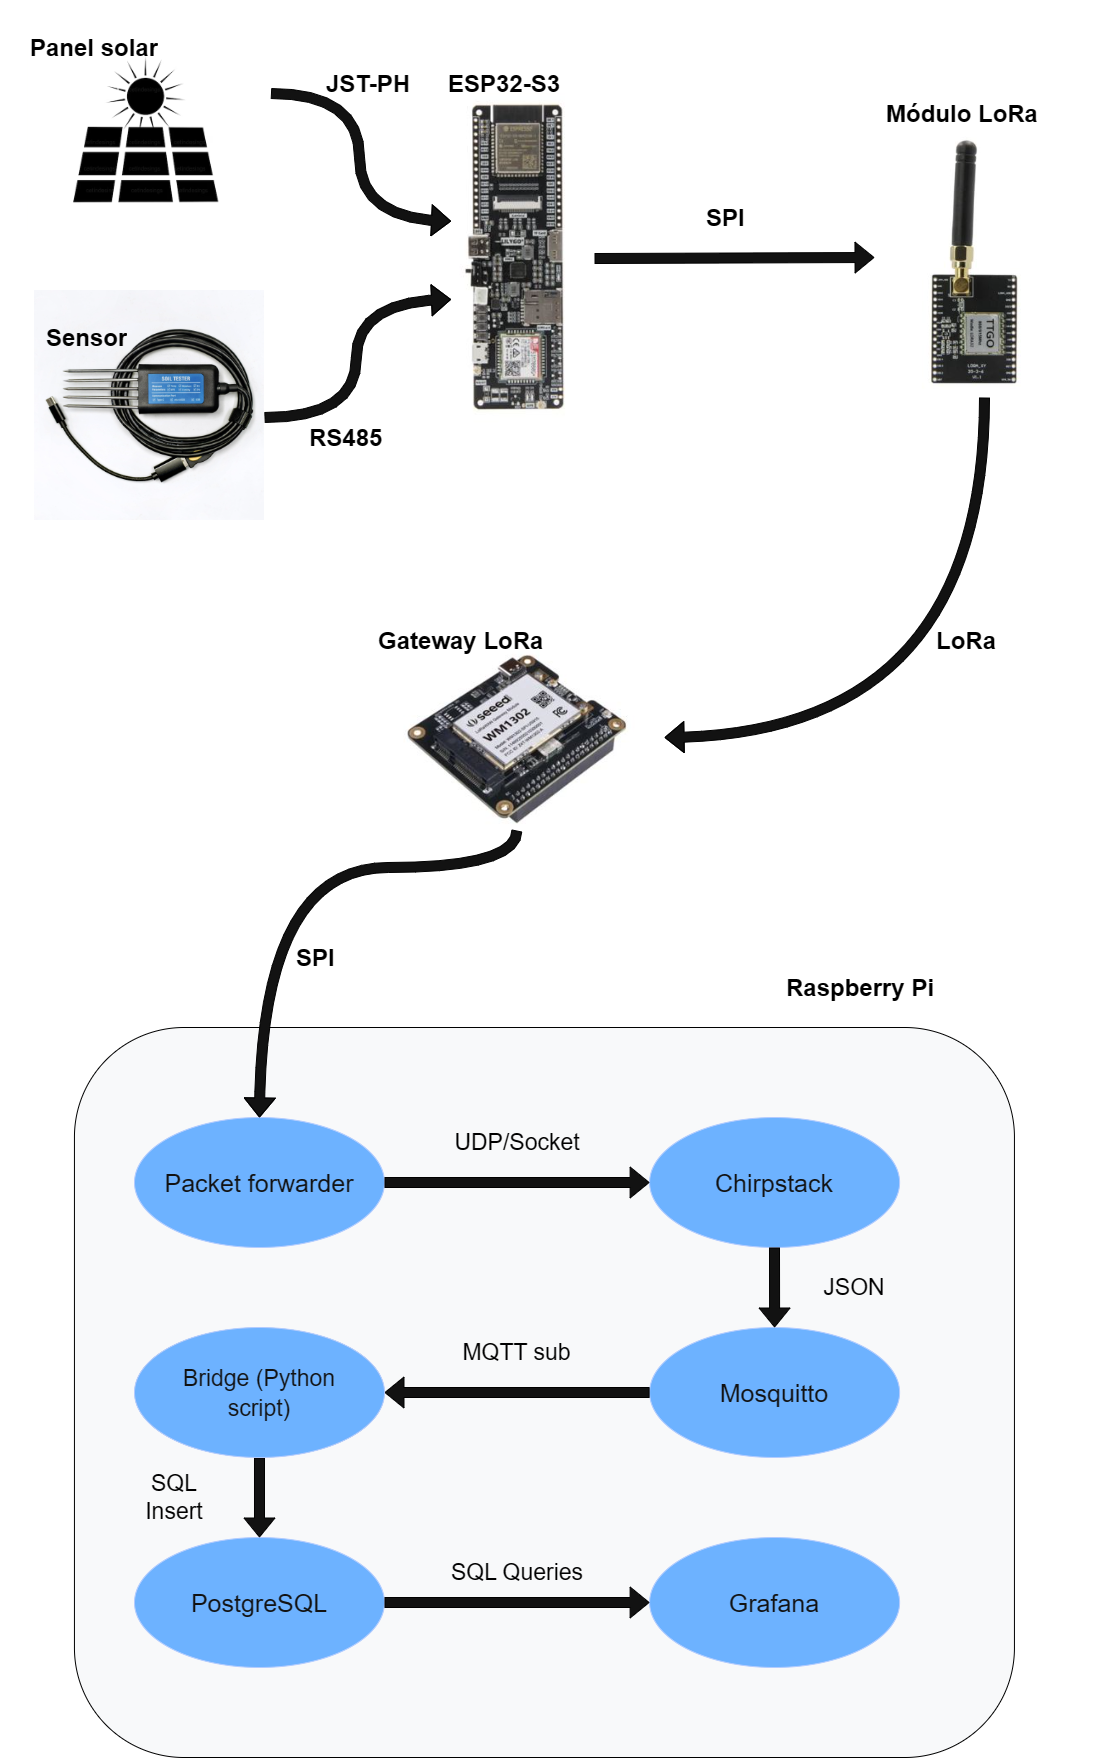
\includegraphics[width=0.72\textwidth]{figs/Diagrama.png}
    \caption{Arquitectura general del sistema extremo a extremo...}
    \label{fig:arquitectura_general}
\end{figure}

\subsection{Visión global y descomposición por capas}

La arquitectura se articula en una jerarquía modular estructurada en cinco capas funcionales diferenciadas:

\begin{enumerate}
    \item \textbf{Capa de percepción e instrumentación de campo:} Compuesta por una sonda industrial multivariable capaz de medir hasta 8 parámetros del sustrato (humedad volumétrica, temperatura, pH, conductividad eléctrica y nutrientes NPK). La comunicación física se canaliza mediante un bus serie industrial diferencial RS-485 inmune al ruido electromagnético, empleando el protocolo maestro-esclavo Modbus RTU para interrogar los registros del sensor bajo demanda.

    \item \textbf{Capa de computación embebida y control (Nodo sensor):} Gobernada por la placa LilyGO T-SIM7080G, provista de un microcontrolador ESP32-S3 de doble núcleo y una unidad de gestión de potencia (PMU AXP2101). Este nodo se encarga de orquestar el ciclo de vida energético del dispositivo, ejecutar la adquisición periódica, gestionar la sincronización horaria mediante el módem GNSS y salvaguardar los registros en memoria volátil retenida (\textit{RTC Slow RAM}) y tarjeta microSD antes de activar el transceptor de radio.

    \item \textbf{Capa de transporte inalámbrico LPWAN (Radio LoRa):} La comunicación de largo alcance se establece entre el módulo transceptor LoRa SX1276 conectado al microcontrolador mediante bus SPI y un concentrador multicanal SX1302 (\textit{Gateway} Seeed WM1302) alojado en la estación receptora. Las tramas se emiten bajo el estándar LoRaWAN en la banda libre europea EU868, empleando activación OTAA y mecanismos de transmisión agrupada por lotes (\textit{batching}) calculados dinámicamente según el factor de dispersión vigente.

    \item \textbf{Capa de pasarela y orquestación de red (Backend local):} Desplegada íntegramente sobre un miniordenador Raspberry Pi conectado físicamente por SPI al concentrador LoRa. La pasarela aloja:
    \begin{itemize}
        \item El demonio \textit{packet forwarder}, encargado de capturar las señales moduladas en el aire y transferirlas como paquetes UDP hacia el servidor de red.
        \item La pila del servidor LoRaWAN ChirpStack, que valida las claves de sesión criptográficas, controla los contadores de trama y ejecuta el decodificador JavaScript del perfil del dispositivo para desempaquetar la carga binaria útil.
        \item El intermediario de mensajería Eclipse Mosquitto (MQTT), que recibe los eventos de subida (\textit{uplink}) publicados por ChirpStack formateados en JSON estructurado.
    \end{itemize}

    \item \textbf{Capa de ingesta, persistencia relacional y analítica:} Un servicio residente en segundo plano programado en Python actúa como pasarela lógica (\textit{bridge}), suscribiéndose al intermediario MQTT, validando las cargas útiles e insertando las mediciones mediante sentencias SQL en un motor relacional PostgreSQL. Por último, la plataforma analítica Grafana consulta directamente las tablas indexadas de la base de datos para renderizar cuadros de mando interactivos y gráficos temporales en tiempo real.
\end{enumerate}

\subsection{Flujo de datos y ciclo de vida de la información}

El ciclo de vida del dato sigue una trazabilidad unidireccional y determinista diseñada para maximizar la integridad metrológica y minimizar el tiempo en el aire (\textit{airtime}) del enlace radio:

\begin{enumerate}
    \item \textbf{Muestreo e interrogación física:} Tras el despertar programado del microcontrolador desde el estado de suspensión profunda (\textit{Deep Sleep}), el PMU AXP2101 activa el carril de alimentación del transceptor RS-485. El ESP32-S3 emite una trama Modbus RTU de lectura (\texttt{Function Code 0x03}) hacia la sonda de suelo, recibiendo los registros binarios que contienen las magnitudes fisicoquímicas instantáneas.
    
    \item \textbf{Estructuración y persistencia de las muestras:} Los valores recibidos se empaquetan en una estructura binaria compacta (\texttt{struct Data} de 19 bytes) con la marca temporal del reloj del ESP32, sincronizado mediante GNSS cuando es posible. Las muestras se añaden a un búfer circular retenido en \textit{RTC Slow RAM}; esta retención no protege ante la pérdida completa de alimentación. La microSD mantiene un histórico JSON Lines (\texttt{.jsonl}), no una cola de reenvío. Solo al finalizar un conjunto por éxito local o segundo fallo se registra una entrada por muestra y se descarta ese conjunto. El excedente excluido del segundo intento por capacidad insuficiente queda para el lote siguiente, sin registro ni descarte anticipados. Si falla SD, se notifica y se descarta igualmente el conjunto finalizado.

    \item \textbf{Decisión de transmisión y conformación de trama:} Al alcanzar el umbral mínimo de cuatro muestras, el firmware enciende la radio y prepara la sesión para consultar la carga útil disponible. El primer envío espera un paquete completo; un lote pendiente se reintenta aunque no alcance la capacidad actual. Si falla la preparación antes de conocer esa capacidad, se seleccionan las cuatro muestras más antiguas. Tras el primer fallo, el estado retenido \texttt{pending\_batch} conserva la identidad, el tamaño y el intento consumido. En el segundo se intenta el prefijo que quepa, dejando el excedente para un lote nuevo; si no puede enviarse ninguna muestra, finaliza el lote pendiente completo. Un aplazamiento por ciclo de trabajo no consume intento ni modifica el conjunto pendiente. El éxito significa que la API de transmisión no devuelve error, sin acreditar recepción remota.

    \item \textbf{Recepción, demodulación y enrutado:} El concentrador Seeed WM1302 demodula la señal de radio en el extremo receptor y el \textit{packet forwarder} remite el paquete crudo mediante sockets UDP a ChirpStack. El servidor de red extrae la carga útil cifrada, autentica el dispositivo y ejecuta el decodificador JavaScript de la aplicación, convirtiendo el bloque binario en objetos JSON que se publican de forma inmediata en el \textit{broker} Mosquitto bajo el tópico correspondiente al dispositivo.

    \item \textbf{Ingesta, almacenamiento relacional y consulta:} El demonio de ingesta en Python, suscrito al \textit{broker} MQTT, consume los mensajes entrantes, desglosa los registros agrupados en muestras atómicas y ejecuta transacciones SQL (\texttt{INSERT}) en PostgreSQL. Los registros se asocian al identificador del nodo y a su marca de tiempo exacta (\texttt{TIMESTAMPTZ}). Grafana consulta de manera asíncrona la base de datos indexada, refrescando las series temporales de humedad, temperatura, electroconductividad y fertilidad NPK en el panel de supervisión.
\end{enumerate}

\subsection{Diagrama de despliegue}

El despliegue físico del sistema se divide en dos emplazamientos claramente diferenciados según sus requerimientos ambientales y energéticos:

\begin{itemize}
    \item \textbf{Emplazamiento de campo (Nodo sensor autónomo):}
    \begin{itemize}
        \item \textbf{Módulo de captación y acondicionamiento:} El sensor multivariable se encuentra enterrado en el perfil radicular del cultivo objetivo, conectado mediante un cable apantallado de par trenzado RS-485 hacia la envolvente del nodo.
        \item \textbf{Caja de control (IP67):} Contiene la placa base LilyGO T-SIM7080G (ESP32-S3), la tarjeta de expansión para el transceptor LoRa SX1276, el circuito transceptor RS-485 y la celda de batería recargable de litio.
        \item \textbf{Alimentación renovable:} Un panel solar fotovoltaico exterior acoplado mecánicamente al mástil se conecta mediante conector JST-PH directamente a la etapa de carga integrada y gobernada por el circuito PMU AXP2101, garantizando un funcionamiento energético autosuficiente y continuo.
    \end{itemize}

    \item \textbf{Infraestructura receptora y de servicios (Estación base):}
    \begin{itemize}
        \item \textbf{Pasarela física:} Formada por una Raspberry Pi montada en riel o encapsulado protector en las inmediaciones o caseta de la explotación, provista de alimentación continua y conectividad de red local.
        \item \textbf{Módulo concentrador LoRa:} La tarjeta Seeed WM1302 acoplada a la interfaz SPI de la Raspberry Pi y conectada a una antena omnidireccional de 868~MHz en el exterior para asegurar cobertura en línea de vista sobre la parcela sensorizada.
        \item \textbf{Entorno de ejecución de servicios:} La Raspberry Pi ejecuta un sistema operativo Linux donde coexisten y se autoinician bajo el gestor de demonios \texttt{systemd} los servicios del \textit{packet forwarder}, ChirpStack, Eclipse Mosquitto, el puente de ingesta en Python, PostgreSQL y el servidor Grafana accesible a través de navegador web en la red local.
    \end{itemize}
\end{itemize}

\section{Diseño hardware del nodo sensor}

En esta sección se detalla la composición física y electrónica del nodo sensor de campo. El enfoque de diseño adoptado combina la integración de módulos comerciales consolidados con el desarrollo de una placa portadora a medida (\textit{Carrier HAT}), reduciendo la complejidad de montaje, eliminando cableados volantes propensos a desconexiones y garantizando la robustez mecánica y eléctrica del dispositivo en campo.

\subsection{Composición e integración de subsistemas}
El diseño hardware parte de una arquitectura modular basada en componentes comerciales de amplia disponibilidad:

\begin{itemize}
    \item \textbf{Módulo de procesamiento y soporte base (LilyGO T-SIM7080G-S3):} Constituye el núcleo computacional del dispositivo. Esta placa integra en un único factor de forma compacto:
    \begin{itemize}
        \item El SoC \textbf{ESP32-S3} (doble núcleo Xtensa LX7), encargado de ejecutar el firmware, gestionar los ciclos de suspensión profunda (\textit{Deep Sleep}) y retener los datos en su memoria interna \texttt{RTC Slow RAM}.
        \item La unidad de gestión de potencia (\textbf{PMU AXP2101}), accesible por bus \text{I\textsuperscript{2}C}, que gobierna la carga de la batería LiPo de 3,7~V, admite entrada directa de panel solar fotovoltaico y permite habilitar o cortar la alimentación de los periféricos.
        \item El módem \textbf{SIM7080G}, del cual se explota exclusivamente su receptor GNSS integrado vía comandos AT sobre UART para calibrar periódicamente la deriva temporal (\textit{drift}) del oscilador RTC.
        \item El zócalo para tarjetas \textbf{microSD}, enlazado al controlador de bajo consumo SD-MMC en modo de 1 bit.
    \end{itemize}
    \item \textbf{Módulo transceptor LoRa (Semtech SX1276):} Módulo de comunicaciones inalámbricas de largo alcance que opera en la banda ISM EU868 (868,1--868,5~MHz). Se comunica con el microcontrolador mediante un bus serie SPI dedicado de cuatro hilos, acompañado de líneas de control y señalización de interrupciones (\texttt{DIO0}, \texttt{DIO1} y \texttt{RST}).
    \item \textbf{Sonda edafológica multivariable de campo:} Instrumento de sensado industrial enterrable que captura las variables fisicoquímicas del terreno (humedad, temperatura, conductividad, pH y macronutrientes NPK). Se comunica mediante par diferencial RS-485 bajo el protocolo Modbus RTU y precisa una tensión continua de alimentación en el rango de 9~V a 12~V.
\end{itemize}

\subsection{Placa de interconexión y acondicionamiento (Carrier HAT)}
Para articular de forma limpia la interconexión entre la placa LilyGO, el transceptor LoRa, la sonda de campo y las fuentes de energía, se diseñó y fabricó una placa portadora (\textit{carrier HAT}) a medida utilizando el entorno \textbf{KiCad EDA v7}.

En la Figura~\ref{fig:esquema_electrico} se presenta el esquema electrónico del circuito desarrollado, el cual aborda la adaptación de señales y la distribución de potencia necesaria para la sonda.

\begin{figure}[htbp]
    \centering
    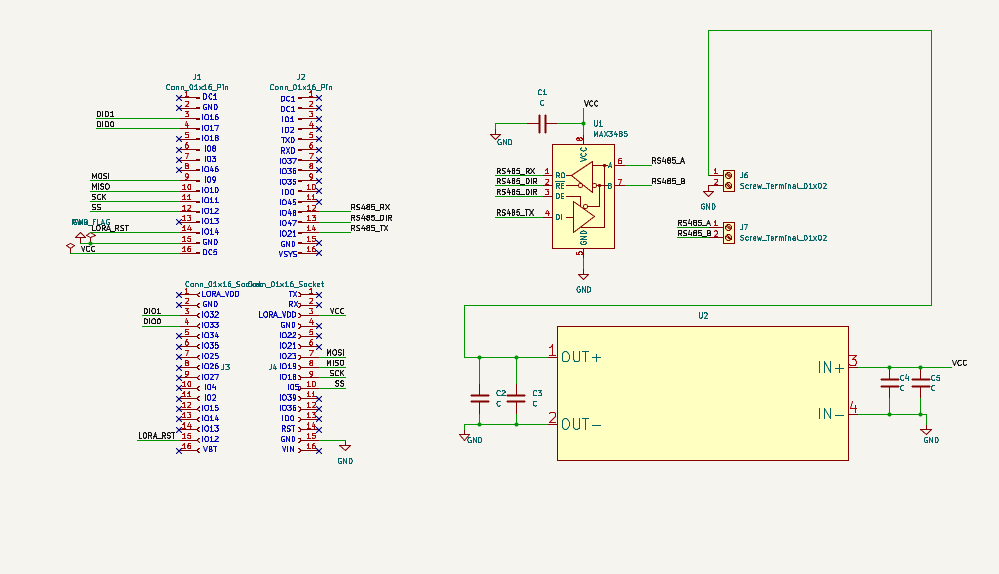
\includegraphics[width=0.95\textwidth]{figs/esquema_electrico.png}
    \caption{Esquema eléctrico del circuito del nodo sensor diseñado en KiCad.}
    \label{fig:esquema_electrico}
\end{figure}

El circuito esquemático resuelve los siguientes aspectos clave:
\begin{itemize}
    \item \textbf{Acondicionamiento y conversión a RS-485 (U1 - MAX3485):} Dado que el microcontrolador opera con niveles lógicos UART TTL a 3,3~V, se implementa el circuito integrado MAX3485 en encapsulado DIP-8 para convertir dichas señales al par diferencial del estándar RS-485. 
    \begin{itemize}
        \item La línea de recepción \texttt{RO} (pin 1) se mapea al pin \texttt{IO46} (\texttt{RS485\_RX}) y la de transmisión \texttt{DI} (pin 4) al pin \texttt{IO21} (\texttt{RS485\_TX}).
        \item Al ser una comunicación semidúplex, los pines de control de recepción ($\overline{\text{RE}}$, activo a nivel bajo) y transmisión ($\text{DE}$, activo a nivel alto) se puentean y quedan gobernados por una única línea de control: \texttt{RS485\_DIR}, conectada al pin \texttt{IO48} del ESP32-S3.
        \item La alimentación \texttt{VCC} del integrado se desacopla mediante el condensador cerámico $C_1$.
    \end{itemize}
    \item \textbf{Elevación de tensión para la sonda (U2 - Step-Up):} Debido a que la tensión nominal de la batería (3,7~V) es insuficiente para excitar la circuitería interna de la sonda NPK, se integra un módulo elevador DC-DC (U2). Su entrada \texttt{IN+} toma el carril \texttt{VCC} desacoplado por los condensadores $C_2$ y $C_3$, entregando por su salida \texttt{OUT+} una tensión regulada adecuada (filtrada por $C_4$ y $C_5$) hacia la borna de alimentación de la sonda.
    \item \textbf{Bornas de conexión de campo (\texttt{J6} y \texttt{J7}):} Terminales de tornillo verdes de dos polos para cableado hacia el exterior. La clema \texttt{J6} suministra la alimentación elevada (\texttt{OUT+}) y la masa (\texttt{GND}) hacia la sonda, mientras que la clema \texttt{J7} conecta el bus diferencial de datos (\texttt{RS485\_A} y \texttt{RS485\_B}).
\end{itemize}

\subsubsection{Mecanismo de acoplamiento físico y apilamiento (Stacking)}
La placa portadora actúa como nexo físico entre los diferentes módulos electrónicos mediante una estructura de apilamiento vertical que optimiza el espacio y prescinde por completo de cables de interconexión. En las Figuras~\ref{fig:pcb_render_top} y~\ref{fig:pcb_render_bottom} se ilustran, respectivamente, la cara superior y la cara inferior de la PCB diseñada:

\begin{figure}[htbp]
    \centering
    \begin{minipage}[t]{0.48\textwidth}
        \centering
        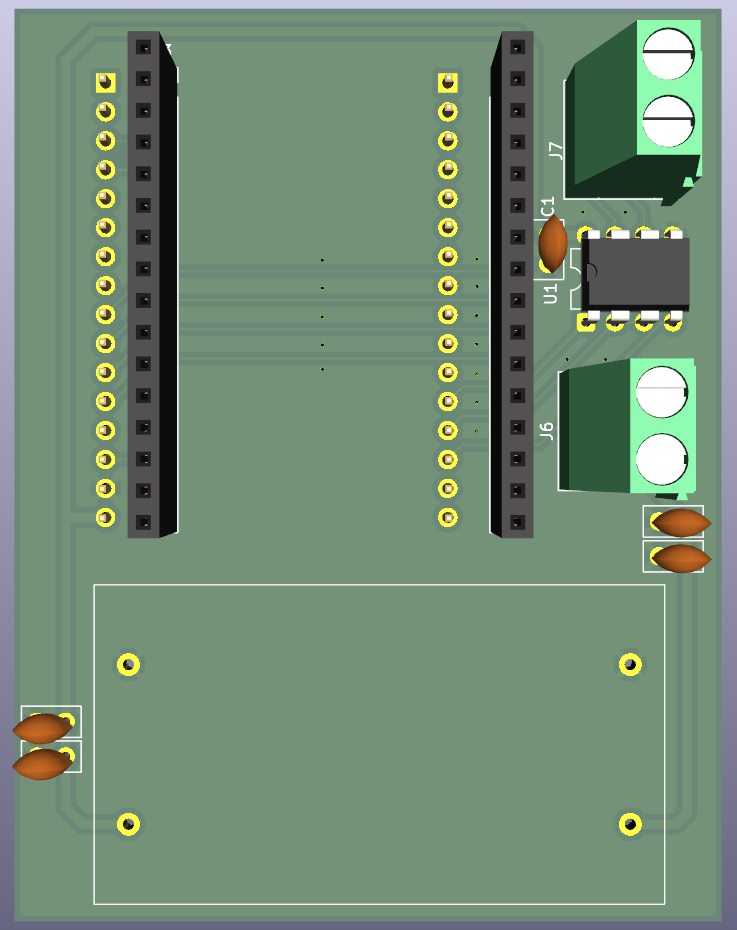
\includegraphics[width=\textwidth]{figs/pcb.png}
        \caption{Cara superior de la PCB: zócalos hembra para LoRa, integrado MAX3485, clemas y filtrado.}
        \label{fig:pcb_render_top}
    \end{minipage}
    \hfill
    \begin{minipage}[t]{0.48\textwidth}
        \centering
        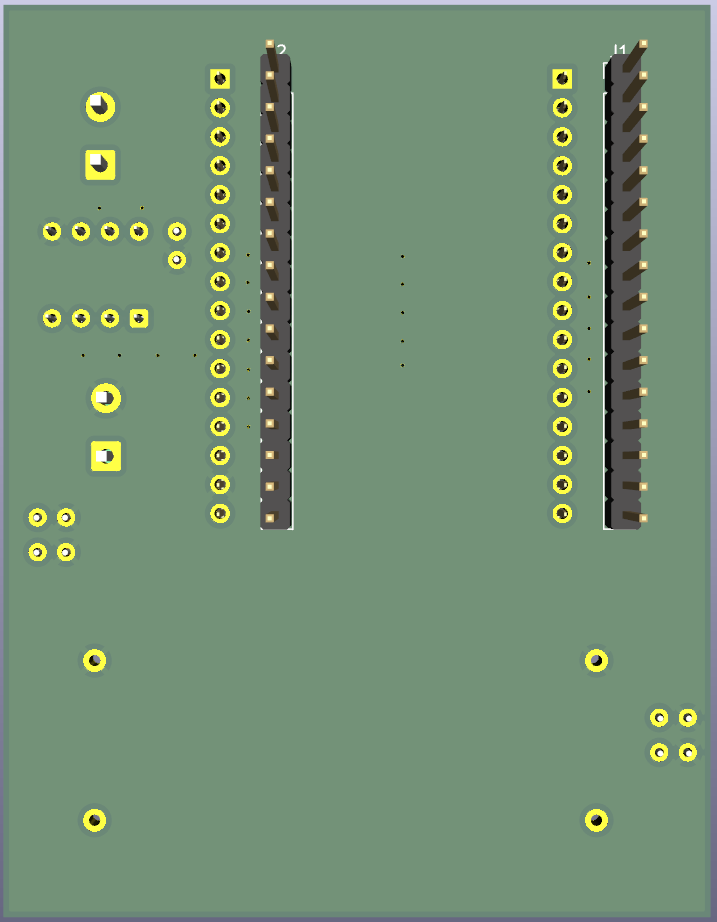
\includegraphics[width=\textwidth]{figs/pcb_bottom.png}
        \caption{Cara inferior de la PCB: tiras de pines macho (J1 y J2) para el acoplamiento directo a la LilyGO.}
        \label{fig:pcb_render_bottom}
    \end{minipage}
\end{figure}

El conexionado modular se fundamenta en las siguientes interfaces:
\begin{itemize}
    \item \textbf{Conexión del HAT a la placa LilyGO (Cara inferior):} En la cara inferior de la PCB se montan dos tiras de pines macho (\texttt{J1} y \texttt{J2}), tal como se aprecia en la Figura~\ref{fig:pcb_render_bottom}. Estas tiras encajan directamente sobre los conectores hembra de la placa LilyGO T-SIM7080G-S3 situada en la base, estableciendo el puente de alimentación (\texttt{VCC}, \texttt{GND}), las líneas de control serie para el MAX3485 y el bus SPI.
    \item \textbf{Conexión del módulo LoRa al HAT (Cara superior):} En la cara superior de la PCB se disponen dos tiras de pines hembra (\texttt{J3} y \texttt{J4}), visibles en la Figura~\ref{fig:pcb_render_top}. Sobre estos conectores hembra se pincha directamente el módulo transceptor LoRa SX1276, recibiendo la alimentación \texttt{VCC} y las líneas SPI y de control procedentes de la placa base a través de pistas dedicadas en la PCB.
    \item \textbf{Alojamiento de la etapa de potencia y filtrado:} En la cara superior se ubica el integrado MAX3485 (U1), los condensadores de desacoplo cerámicos y la huella serigrafiada con cuatro taladros de fijación para soldar el módulo elevador DC-DC (U2), manteniéndolo físicamente próximo a la clema de salida de alimentación (J6).
\end{itemize}

Este diseño de doble apilamiento (\textit{sandwich}) asegura que todo el conjunto quede ensamblado de forma compacta y rígida, facilitando su inserción en la caja estanca con certificación IP67.
% \begin{figure}[htbp]
%     \centering
%     \includegraphics[width=0.85\textwidth]{figuras/bloques_hardware.pdf}
%     \caption{Diagrama de bloques de la arquitectura hardware del nodo sensor.}
%     \label{fig:bloques_hardware}
% \end{figure}

\subsection{Etapa de alimentación y gestión de potencia}
Para asegurar una autonomía operativa indefinida sin recurrir a tendido eléctrico ni sustitución manual de baterías, el esquema de alimentación se apoya en un sistema de recolección fotovoltaica:

\begin{itemize}
    \item \textbf{Almacenamiento químico e interfaz solar:} El nodo integra una celda de polímero de litio (LiPo) de 3,7~V (2000~mAh) y una entrada para panel solar fotovoltaico exterior (rango de 4,4~V a 6,0~V), conectada a través de terminales JST-PH directamente a la etapa de carga lineal CC/CV del PMU AXP2101.
    \item \textbf{Monitoreo y protección ante sobredescarga:} Antes de iniciar los periféricos, el firmware consulta el porcentaje de batería que reporta la PMU. Si el valor es válido y está por debajo de \texttt{CRITICAL\_LEVEL} (10\,\%), el ciclo se aborta y el nodo vuelve a suspensión profunda. El firmware actual no comprueba aquí un umbral de tensión de 3,4~V.
    \item \textbf{Conmutación de carriles de potencia (\textit{Power Gating}):} Durante los intervalos de suspensión profunda (\textit{Deep Sleep}), el microcontrolador instruye al AXP2101 para que deshabilite los carriles LDO y DC-DC asociados a los elementos de mayor consumo (radio LoRa, módem y tarjeta SD). La memoria \texttt{RTC Slow RAM} conserva las lecturas en tránsito y el estado de sesión mientras el dominio RTC permanezca alimentado; esta retención no es persistente ante una pérdida completa de alimentación.
\end{itemize}

\subsection{Acondicionamiento del bus de campo RS-485}
La integración de la sonda industrial edafológica multivariable requiere adaptar los niveles lógicos del procesador a una línea diferencial semidúplex y suministrar la tensión de excitación adecuada:

\begin{itemize}
    \item \textbf{Transceptor diferencial (U1 - MAX3485):} Se implementa un circuito integrado MAX3485 en encapsulado DIP-8 alimentado por el carril de 3,3~V (\texttt{VCC}) y desacoplado localmente mediante el condensador cerámico de lenteja $C_1$. Su pin de recepción \texttt{RO} (pin 1) se conecta a la línea \texttt{RS485\_RX} (\texttt{IO46}) del microcontrolador, mientras que el pin de entrada de transmisión \texttt{DI} (pin 4) se conecta a la línea \texttt{RS485\_TX} (\texttt{IO21}).
    \item \textbf{Control del flujo de datos (\textit{Direction Control}):} Para operar en modo semidúplex sobre el par trenzado, los pines de habilitación de recepción ($\overline{\text{RE}}$, pin 2, activo a nivel bajo) y de transmisión ($\text{DE}$, pin 3, activo a nivel alto) se encuentran puenteados y gobernados por la línea de control \texttt{RS485\_DIR}, conectada al pin \texttt{IO48} del microcontrolador. Un nivel lógico alto en \texttt{IO48} conmuta el transceptor a modo de emisión para lanzar la trama de petición Modbus RTU, mientras que un nivel bajo lo devuelve al modo de escucha para recibir la respuesta de la sonda.
    \item \textbf{Elevación de tensión para la sonda (U2):} La sonda multivariable precisa una tensión de alimentación continua de 9 a 12~V, incompatible con el nivel nominal de la batería. Para ello, se incorpora un módulo elevador DC-DC \textit{Step-Up} (U2). La entrada \texttt{IN+} (pin 1) se alimenta desde el carril \texttt{VCC}, desacoplada en paralelo por los condensadores $C_2$ y $C_3$, mientras que la salida regulada de alta tensión \texttt{OUT+} (pin 3) se filtra mediante el par capacitivo $C_4$ y $C_5$.
    \item \textbf{Bornas de conexión externa (J6 y J7):} La interconexión física hacia el exterior de la caja se realiza mediante dos clemas de tornillo de paso estándar:
    \begin{itemize}
        \item \textbf{Clema J6 (Alimentación de la sonda):} El terminal 1 conecta la tensión elevada \texttt{OUT+} procedente de U2 y el terminal 2 conecta el retorno al plano de masa común (\texttt{GND}).
        \item \textbf{Clema J7 (Bus diferencial de datos):} El terminal 1 conecta la línea diferencial no inversora \texttt{RS485\_A} (pin 6 de U1) y el terminal 2 conecta la línea inversora \texttt{RS485\_B} (pin 7 de U1).
    \end{itemize}
\end{itemize}

\subsection{Diseño y ruteo de la placa de circuito impreso (PCB)}
El diseño esquemático y el trazado de la placa de circuito impreso tipo \textit{carrier HAT} se llevaron a cabo utilizando el entorno \textbf{KiCad EDA v7}. La placa actúa como chasis de integración física, permitiendo el conexionado directo entre el módulo de control LilyGO, el transceptor de radio y los periféricos de potencia:

\begin{itemize}
    \item \textbf{Topología física y apilamiento (\textit{Stacking}):} En la Figura~\ref{fig:pcb_nodo_3d} se muestra el renderizado tridimensional de la PCB desarrollada. La placa aloja en su cara superior dos pares de tiras de pines hembra:
    \begin{itemize}
        \item Tiras externas (\texttt{J1} y \texttt{J2}): Alojan la placa LilyGO T-SIM7080G-S3, enrutando las señales de alimentación (\texttt{VCC}, \texttt{GND}), el bus de control RS-485 (\texttt{IO46}, \texttt{IO48}, \texttt{IO21}) y el bus SPI de comunicaciones.
        \item Tiras internas (\texttt{J3} y \texttt{J4}): Permiten pinchar el módulo transceptor LoRa SX1276 (\texttt{J\_LORA}), conectando directamente sus líneas SPI (\texttt{MOSI}, \texttt{MISO}, \texttt{SCK}, \texttt{SS}) y pines de señal (\texttt{DIO0}, \texttt{DIO1}, \texttt{LORA\_RST}).
    \end{itemize}
    \item \textbf{Emplazamiento de potencia y filtrado capacitivo:} En la mitad inferior de la PCB se reservó una huella con cuatro taladros pasantes metalizados para el montaje mecánico del módulo elevador DC-DC (U2). Inmediatamente adyacentes a las entradas y salidas de potencia se rutearon pares de condensadores de filtrado en paralelo ($C_2/C_3$ a la entrada de U2, y $C_4/C_5$ a la salida hacia la clema J6) para absorber picos transitorios y rizado de conmutación.
    \item \textbf{Estrategia de desacoplo y planos de masa:} Para evitar interferencias en el receptor LoRa y prevenir caídas de tensión bruscas durante las ráfagas de transmisión de RF, se empleó una PCB de doble capa con un plano inferior de masa (\texttt{GND}) continuo. Se mantuvo una separación física deliberada entre la zona de conmutación de potencia (U2 y J6) y la zona digital/RF (MAX3485, conectores SPI de radio y bus de datos J7), reduciendo bucles de retorno y garantizando una alta relación señal/ruido en las lecturas analógicas y diferenciales.
\end{itemize}

% \begin{figure}[htbp]
%     \centering
%     \includegraphics[width=0.6\textwidth]{figuras/pcb_render_3d.png}
%     \caption{Renderizado tridimensional de la PCB HAT del nodo sensor diseñada en KiCad EDA.}
%     \label{fig:pcb_nodo_3d}
% \end{figure}

\section{Diseño del software embebido (Firmware)}

El firmware del nodo sensor ha sido desarrollado en lenguaje C++ utilizando un enfoque orientado a objetos, encapsulando las funcionalidades del hardware en módulos estáticos independientes (\texttt{Power}, \texttt{Clock}, \texttt{Lora}, \texttt{Modem}, \texttt{Sensor} y \texttt{SD}). El diseño lógico prioriza la eficiencia energética, la retención de datos en memoria no volátil y la optimización del tiempo de uso del espectro radioeléctrico.

\subsection{Ciclo de vida y máquina de estados del nodo}
La arquitectura de ejecución del nodo prescinde del tradicional bucle continuo (\texttt{loop()}) a favor de una máquina de estados lineal ejecutada íntegramente dentro de la rutina de inicialización \texttt{setup()}. Este paradigma garantiza que el microcontrolador permanezca activo estrictamente el tiempo necesario antes de transicionar al estado de suspensión profunda (\textit{Deep Sleep}):

\begin{itemize}
    \item \textbf{Arranque y evaluación energética:} Al despertar, el sistema habilita el hardware mínimo y evalúa el porcentaje de batería mediante la unidad de gestión de potencia (\texttt{PMU}). Si el nivel energético es inferior al umbral crítico (\texttt{CRITICAL\_LEVEL}), el nodo aborta la ejecución y vuelve a dormir para proteger la integridad química de la celda de litio.
    \item \textbf{Sincronización y adquisición:} Se inicializa un búfer circular en memoria retenida (\texttt{rtc\_buffer}) y se evalúa si el sistema requiere sincronización horaria absoluta (arranque en frío o si ha transcurrido más de un día desde la última calibración). A continuación, se captura el porcentaje de batería y la marca de tiempo, se energiza la sonda de campo, se realiza la lectura y se apaga inmediatamente la instrumentación para ahorrar energía.
    \item \textbf{Transición a reposo profundo:} Tras evaluar las condiciones de transmisión y persistir los datos, el nodo invoca la rutina \texttt{Power::enterDeepSleep()}. Esta función desconecta por hardware los reguladores del módem, la tarjeta SD y los periféricos de 3,3~V (carriles DC3, BLDO2, ALDO3 y DC5) y reinicia los pines de control pertinentes. El intervalo nominal es de 600\,s (10 minutos), definido por \texttt{DEEP\_SLEEP\_TIME\_S}; la expresión correspondiente es \texttt{600 * 1000000ULL} microsegundos. El tiempo activo se añade a la suspensión, por lo que no se trata de un periodo exacto de adquisición de 600\,s.
\end{itemize}

\subsection{Adquisición de campo y sincronización temporal}
Para garantizar la precisión de las series temporales y la integridad de las mediciones, el firmware integra rutinas específicas de interrogación industrial y calibración satelital:

\begin{itemize}
    \item \textbf{Interrogación Modbus RTU:} La captura de datos edafológicos se encapsula en la clase \texttt{Sensor}. Se excita el pin de control de dirección (\texttt{RS485\_DIR1}) y se transmite una trama de petición (\texttt{0x01, 0x03, 0x00, 0x00, 0x00, 0x07, 0x04, 0x08}) correspondiente a la lectura de registros de retención (\textit{Holding Registers}). El sistema queda a la escucha esperando una trama binaria de respuesta de 19 bytes que contiene las variables empaquetadas, retornando un estado de error si se excede el temporizador \texttt{SENSOR\_READ\_TIMEOUT}.
    \item \textbf{Sincronización horaria absoluta GNSS:} A través de la clase \texttt{Clock}, el nodo intenta corregir la deriva de su reloj de tiempo real (RTC) consultando al módem SIM7080G. La búsqueda de un \textit{fix} dispone de un máximo de 300\,s, al que se suman los tiempos de arranque y apagado del módem. De la respuesta \texttt{AT+CGNSINF} se comprueban el estado de \textit{fix} y el formato de fecha; la conversión fija explícitamente el huso UTC y rechaza fechas que se normalicen a otro día. La marca se aplica mediante \texttt{settimeofday}, comprobando su resultado, y \texttt{last\_sync\_timestamp} conserva la fecha del último éxito en RTC. La sincronización vuelve a vencer a las 24 horas (\texttt{SECONDS\_DAY = 86400}); los fallos se reintentan tras al menos 600\,s desde su finalización. Si no se obtiene hora válida, el muestreo, el envío y el registro continúan con el reloj del ESP32, sin garantizar UTC real hasta una sincronización posterior. No se corrigen retrospectivamente las marcas de las muestras ya adquiridas.
\end{itemize}

\subsection{Estructura de datos y persistencia multinivel}
El manejo de los datos muestreados se ha diseñado para minimizar los ciclos de escritura en almacenamiento no volátil y agilizar el empaquetado binario:

\begin{itemize}
    \item \textbf{Retención volátil de ultrabajo consumo:} Las muestras se encolan inicialmente en un búfer circular (\texttt{rtc\_buffer}) declarado con el atributo \texttt{RTC\_DATA\_ATTR}, lo que ubica esta estructura en la memoria \texttt{RTC Slow RAM} del microcontrolador. Esto permite acumular lecturas de forma continua durante los periodos de \textit{Deep Sleep} sin penalización de tiempo ni desgaste mecánico.
    \item \textbf{Validación del contexto retenido:} La firma \texttt{RTC\_BUFFER\_MAGIC = 0x52544247u} identifica el contexto del búfer y del lote pendiente. Si no coincide al arrancar, se reinician ambos y el contador de cabecera. La firma permite descartar un contexto incompatible, pero no comprueba por sí sola la integridad de todas las muestras ni recupera datos tras pérdida completa de alimentación.
    \item \textbf{Auditoría y persistencia local:} Cada conjunto finalizado se registra mediante una línea JSON por muestra en el archivo de la fecha del reloj del ESP32 al escribir, conservando las marcas originales. Tras éxito local o segundo fallo se descarta solo ese conjunto; el excedente reservado para el lote siguiente permanece en RTC. Si falla SD, se notifica y se descarta igualmente el conjunto finalizado. No se reenvía desde SD. No se garantiza atomicidad entre la escritura y la actualización de RTC si se interrumpe la alimentación durante la finalización.
\end{itemize}

\subsection{Estrategia de transmisión por lotes (Batching) y sesión LoRaWAN}
El subsistema de radio, gobernado por la clase \texttt{Lora}, implementa mecanismos avanzados para optimizar el tiempo de emisión en el aire (\textit{Airtime}) y acatar las normativas europeas sobre el ciclo de trabajo:

\begin{itemize}
    \item \textbf{Agrupación dinámica de lecturas (\textit{Batching}):} La capacidad se calcula mediante \texttt{node.getMaxPayloadLen() / sizeof(Data)} e incluye las restricciones del estado MAC y del \textit{Data Rate}. La primera transmisión requiere un lote completo según esa capacidad. La función \texttt{sendBatch()} recibe además un límite de muestras, para no incorporar al reintento las nuevas lecturas acumuladas.
    \item \textbf{Identidad y reintentos de envío:} \texttt{pending\_batch} retiene en RTC la referencia de la primera muestra, su conteo y los intentos consumidos. La referencia procede de \texttt{rtc\_buffer\_front\_id}, que avanza únicamente al descartar muestras de cabecera; no depende del timestamp. Un fallo de preparación de radio o sesión consume intento; \texttt{RADIOLIB\_ERR\_UPLINK\_UNAVAILABLE} aplaza la operación sin consumirlo. Tras el primer fallo se conserva el lote. Si la capacidad baja en el segundo, se finaliza solo el prefijo intentado, por éxito o segundo fallo, y el excedente conserva sus datos para un lote nuevo con dos intentos propios. Por ejemplo, de ocho muestras pendientes, si caben cinco se finalizan esas cinco y se reservan tres. Si no cabe ninguna o vuelve a fallar la preparación, se finaliza el lote pendiente completo. La SD se invoca solo al finalizar, no tras el primer fallo.
    \item \textbf{Preservación de la sesión OTAA:} Para evitar costosas renegociaciones de red (procedimiento \textit{Join}) tras cada ciclo de \textit{Deep Sleep}, el estado completo de la pila LoRaWAN (variables de sesión \texttt{lorawanSession} y contadores criptográficos \texttt{lorawanNonces}) se exporta y retiene en la memoria \texttt{RTC\_DATA\_ATTR}. 
    \item \textbf{Tolerancia a fallos de energía prolongados:} Adicionalmente, los contadores de tramas (\texttt{nonces}) se guardan de forma permanente en la memoria Flash (NVS) mediante la librería \texttt{Preferences}, previniendo ataques de repetición y desincronizaciones graves con el servidor de red \texttt{ChirpStack} ante un agotamiento total de la celda de litio.
    % TODO: Contrastar si el DevNonce debe persistirse en NVS tras un Join OTAA exitoso y validar el comportamiento con un arranque en frío.
\end{itemize}


\section{Diseño de la infraestructura de red y comunicaciones}
\subsection{Topología LoRaWAN y parámetros de modulación}
% Configuración de la banda regional EU868, canales, anchos de banda y esquema de activación OTAA.
\subsection{Preservación de sesión de red entre ciclos de reposo}
% Almacenamiento de claves criptográficas (NwkSKey, AppSKey) y contadores (FCntUp) en memoria retenida.
\subsection{Diseño del protocolo de mensajería interna (MQTT)}
% Jerarquía de topics para publicación de telemetría y eventos de red en ChirpStack.

\section{Diseño del backend y almacenamiento}
\subsection{Arquitectura desacoplada de la estación receptora}
% Separación de roles: Packet Forwarder, ChirpStack v4, Eclipse Mosquitto y servicio puente de ingesta.
\subsection{Diseño del servicio de ingesta y transformación}
% Lógica del demonio en Python para suscripción MQTT, validación de carga y persistencia.
\subsection{Modelo relacional de datos}
% Modelo Entidad-Relación y esquema de base de datos en PostgreSQL.
\subsection{Estrategia de indexación y optimización de consultas temporales}
% Definición de índices B-Tree sobre (device_eui, recorded_at DESC) y tipos TIMESTAMPTZ.

\section{Diseño de la plataforma de visualización}
\subsection{Estructura de cuadros de mando en Grafana}
% Definición de métricas agronómicas: paneles de series temporales, diagramas NPK y salud del nodo.
\subsection{Diseño de consultas analíticas y alertas}
% Definición conceptual de las sentencias SQL de extracción y umbrales de alerta de batería baja.